\section{Discussion}
\label{section:discussion}
In the Discussion, the experimental results are interpreted and analysed. The discussion is organized into three 
main subsections similar with Section \ref{section:results}, which are analysis of model performance, uncertainty 
estimation, and domain transfer. Subsection \ref{section:AMP} focuses on evaluating the model performance in 
comparison with other models. Subsection \ref{section:AUE} examines how uncertainty estimation may enhance the 
robustness of the model for USVs. Subsection \ref{section:ADT} analyses the generalization capabilities of 
Bayesian SegNet Method.

\subsection{Analysis of Model Performance}
\label{section:AMP}
Firstly, the training and evaluation curves presented in Fig.\ref{fig:nbs-mastr1325-perf} do not conclusively 
demonstrate that the SegNet model has converged, nor do they definitively indicate that further training would 
result in overfitting. Theoretically, continued training could be viable. However, the decision to cease further 
training of the SegNet model was predicated on the excessive computational resources consumed by the process. 
According to the log files, training for 200 epochs with a batch size of 4 on an NVIDIA 4090D GPU consumed 
approximately 9.982 hrs, with an average time of 179.67 seconds per epoch. Further training would likely yield 
only marginal improvements whilst requiring significantly more computational resources, rendering it suboptimal 
from a cost-benefit perspective. 

In contrast, the Bayesian SegNet architecture, owing to its use of MC dropout which mitigates overfitting, can 
theoretically be trained indefinitely. In practice, training for 1000 epochs with a batch size of 1 required 12.6 
hours, with an average of 45.36 seconds per epoch. This reduction in computational time is attributable to the 
dropout process severing certain connections, thereby economising on calculations. As evident from Fig.
\ref{fig:bs-mastr1325-perf}, the model appears to have converged around epoch 300, with the subsequent 700 epochs 
yielding relatively limited improvements.

The more severe instability observed in the evaluation curves of the non-Bayesian SegNet model may be mainly 
attributed to the relatively large learning rate during training, which leads to fluctuations in the performance 
metrics during evaluation. In contrast, the Bayesian SegNet model makes the evaluation curve smoother through the 
implementation of smaller learning rate and MC dropout.

Additionally, this study evaluates the performances of models using different softmax thresholds based on the 
evaluation metrics in Fig.\ref{fig:eval-threshold}. The results indicate that while SegNet demonstrates higher 
precision than Bayesian SegNet when the threshold is low, Bayesian SegNet generally outperforms SegNet in other 
scenarios. The lower precision of Bayesian SegNet at lower thresholds may be attributed to the prior distribution, 
which potentially increases the probabilistic weighting of obstacles. This adjustment likely encourages Bayesian 
SegNet to classify more objects as obstacles, resulting in a higher $\mathbf{FP_r}$. 

The evaluation of the model performance has certain limitations. Firstly, it would be advantageous to experiment 
with varying batch sizes during the training of the Bayesian SegNet model to identify the optimal configuration. 
Secondly, exploring modifications to the prior distribution within the Bayesian SegNet algorithm could be valuable 
in determining whether it can enhance precision at lower softmax thresholds. Despite these considerations, the 
Bayesian SegNet model overall demonstrates superior performance when compared to SegNet and other models, making 
it particularly well-suited for maritime semantic segmentation.

\subsection{Analysis of Uncertainty Estimation}
\label{section:AUE}
Compared to the approximate confidence generated by softmax function, Bayesian SegNet offers a more accurate 
uncertainty estimation. Since the softmax probabilistic cannot be directly compared with uncertainty measurands, 
they are converted into entropy and then compared with aleatoric uncertainty, which is also in the form of entropy. 
Subtracting aleatoric uncertainty from the softmax entropy reveals that entropy at the obstacle edges during semantic 
segmentation is notably higher with the softmax function. Owing to resolution limitations, boundaries are difficult 
to delineate, resulting in high uncertainty in these regions. However, aleatoric uncertainty provides a smoother 
transition by better quantifying this uncertainty. As illustrated in Fig.\ref{fig:entropy}, the pixel with the 
highest entropy has a softmax entropy of 0.92025, while the entropy calculated from aleatoric uncertainty is only 
0.4581. The red dots in the image highlight points where there is a significant difference between the two entropy 
values.
% figure
\begin{figure}[ht!]
    \centering
        \centering
        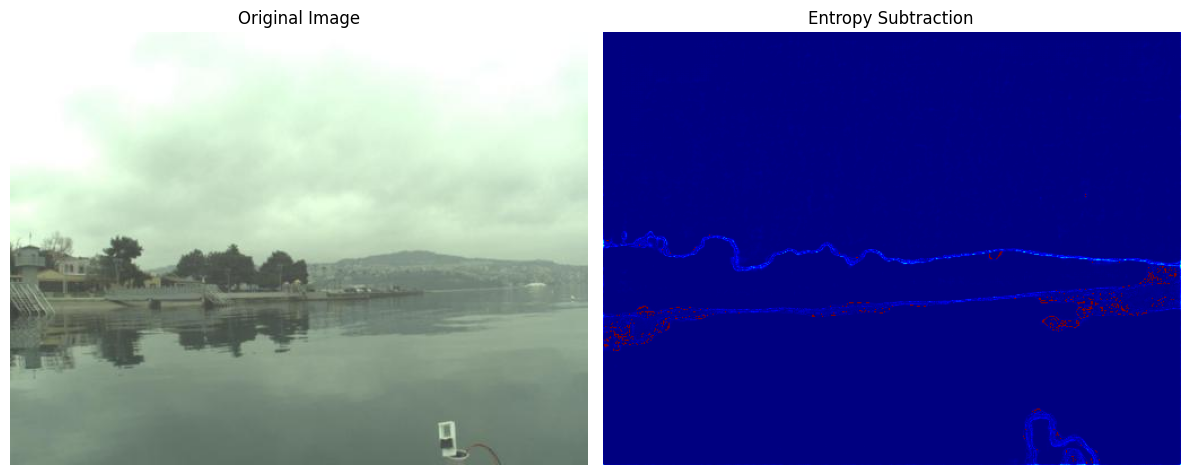
\includegraphics[width=0.9\textwidth]{figures/MaSTr1325/entropy.png}
    \caption{Entropy subtraction for uncertainty estimation comparison.}
    \label{fig:entropy}
\end{figure}

Moreover, there are certain issues associated with uncertainty estimation. Firstly, there is significant overlap 
between epistemic uncertainty and heteroscedastic aleatoric uncertainty, as illustrated in Fig.
\ref{fig:bs-mastr1325-disp}. The underlying reasons for this overlap can be analysed from the perspective of the 
USV image itself and the ground truth labels used in training. 

From the perspective of USV images, at the edges of semantic segmentation, the model struggles to assign a 
definitive label to a pixel due to resolution limitations. This results in high epistemic uncertainty. 
Additionally, these edge regions are more susceptible to factors like lighting, which increases the inherent 
noise during observation, leading to higher heteroscedastic aleatoric uncertainty.

From the perspective of dataset labelling, edge regions in the images are labelled as class 4, which is the unknown 
categories. In the model's prior, class 4 is assigned a value of 0, meaning the model has limited understanding of 
these regions, which results in higher epistemic uncertainty. Correspondingly, due to heteroscedastic aleatoric 
uncertainty capturing inherent noise from the data, these unlabelled regions inherently possess a high degree of 
uncertainty, thus leading to greater heteroscedastic aleatoric uncertainty.

Moreover, leveraging uncertainty to assist USVs in visual enhancement and further improve their robustness remains 
a challenge. As shown in Table \ref{tab:uncertainty-threshold}, setting a threshold for epistemic uncertainty can 
enhance segmentation performance. However, the selection of this specific threshold lacks mathematical justification 
and cannot be quantitatively determined.

\subsection{Analysis of Domain Transfer}
\label{section:ADT}
Bayesian SegNet demonstrated outstanding performance in generalization capabilities evaluation. In the results, 
the OASIs dataset was divided into six subcategories. This section will analyse the performance of Bayesian and 
non-Bayesian models across these six subcategories and compare their generalization performance with the SegNet 
model, which was also trained on the MaSTr1325 dataset and evaluated on the SMD dataset.

In the multi-class scatter plot (Fig.\ref{fig:domain-transfer-disp}), the segmentation performance of various 
architectures across different subcategories is presented. The Bayesian SegNet architecture demonstrates strong 
performance for the USV perspective on the OASIs dataset, achieving an average $\mathbf{F1}$ of 70.21\% across the 
three types, which indicates a balance between precision and recall in semantic segmentation. The semantic segmentations 
of three types are illustrated in Fig.\ref{fig:bs-oasis-usv}. Conversely, when applied to semantic segmentation 
of cargo ship images in the OASIs dataset, the $\mathbf{F1}$ of the Bayesian SegNet architecture shows a decline by 
approximately 30\%. This reduction can be attributed to the lack of similar scenario in the MaSTr1325 dataset. 
The semantic segmentation results for cargo ship perspectives, as shown in Fig.\ref{fig:bs-oasis-cargo}, 
highlight the difficulty of performing inference with BDL on completely novel perspectives, resulting in 
suboptimal performance. However, in these scenarios, the algorithm yields high uncertainty estimates, which 
contribute to the robustness of the USV when navigating entirely novel environments. 
% figure
\begin{figure}[ht!]
    \centering
        \centering
        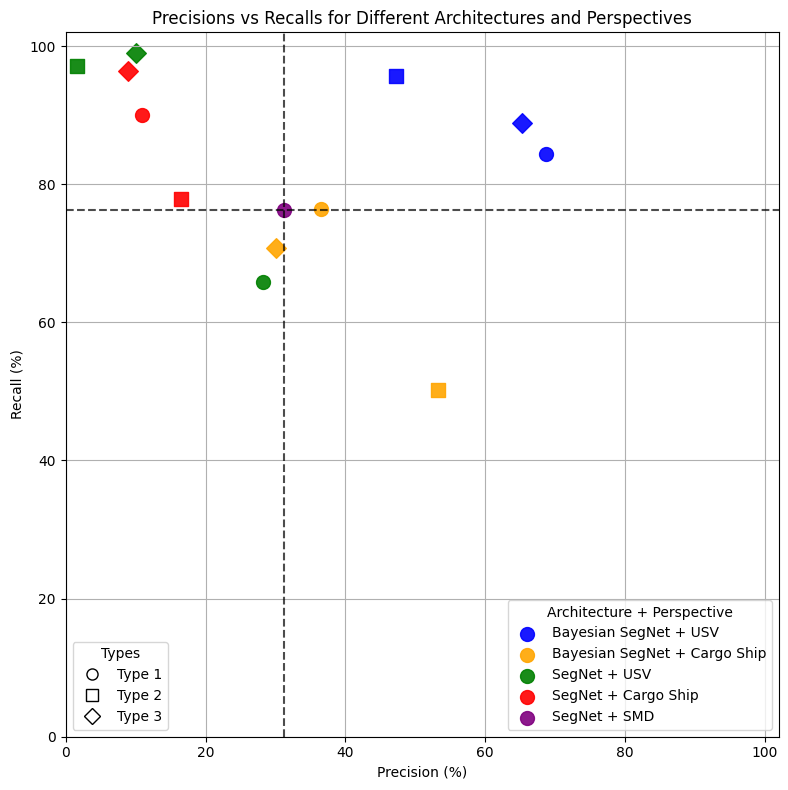
\includegraphics[width=0.5\textwidth]{figures/OASIs/domain-tranfer-PrRe.png}
    \caption{Domain transfer of different architecture and subcategories.}
    \label{fig:domain-transfer-disp}
\end{figure}
% figure
\begin{figure}[t!]
    \centering
        \centering
        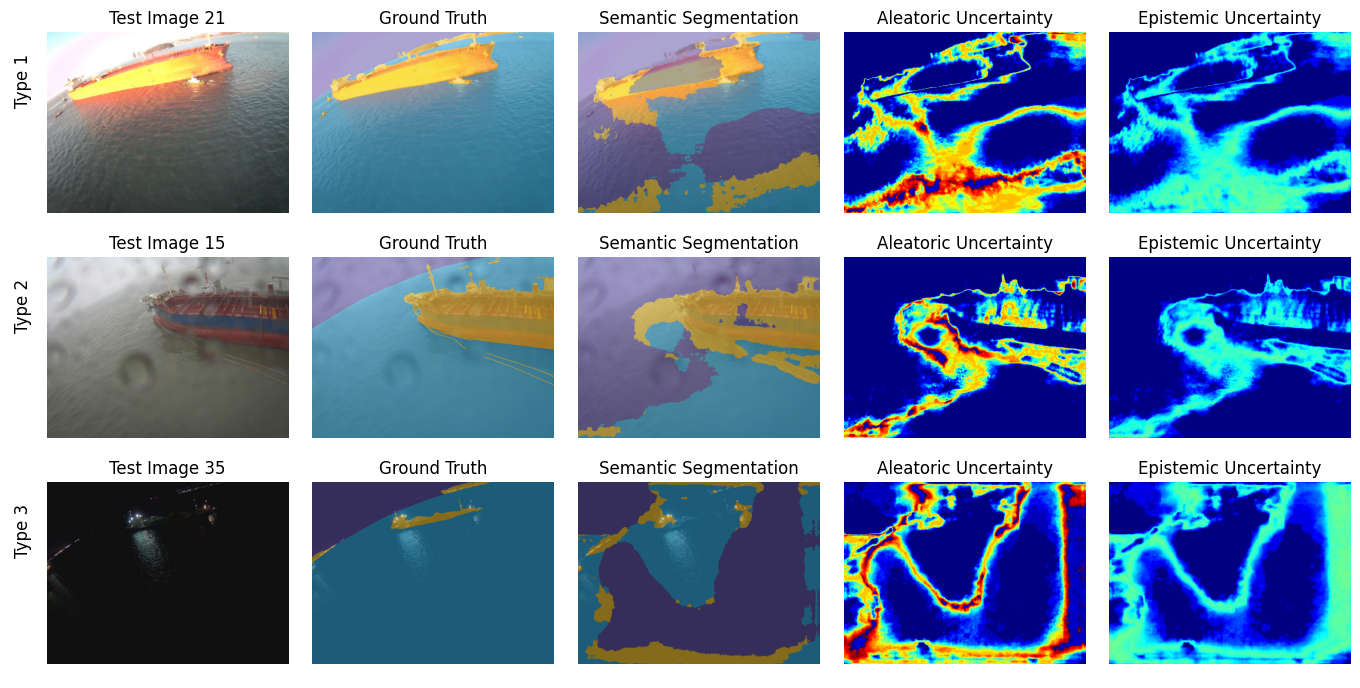
\includegraphics[width=0.9\textwidth]{figures/OASIs/BayesianSegNet-cargo-panel.png}
    \caption{Bayesian SegNet performance evaluation on cargo ship perspective.}
    \label{fig:bs-oasis-cargo}
\end{figure}

Although this study primarily focuses on USVs, the cargo ship perspective was included as a reference due to the 
limited number of USV perspective images available in the OASIs dataset for types 2 and 3. This inclusion serves 
as a reference point and facilitates further investigation into the model's inference capabilities in novel scenarios. 
% figure
\begin{figure}[ht!]
    \centering
    % subfig1
    \begin{subfigure}[h]{0.49\textwidth} \centering
        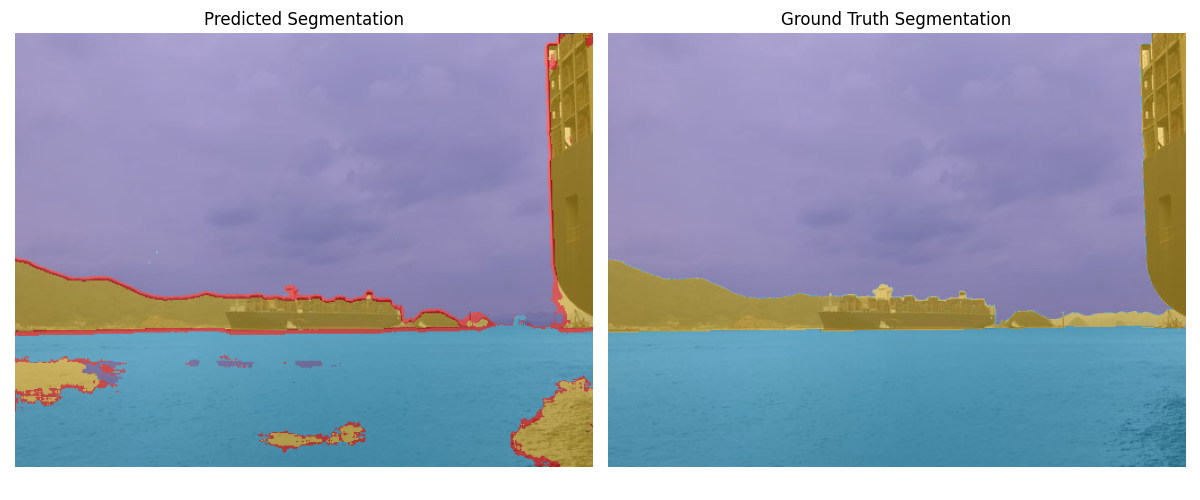
\includegraphics[width=0.99\textwidth]{figures/OASIs/SegNet-type1-91.png}
        \caption{}
    \end{subfigure} \hspace{-10mm}
    % subfig2
    \begin{subfigure}[h]{0.49\textwidth} \centering
        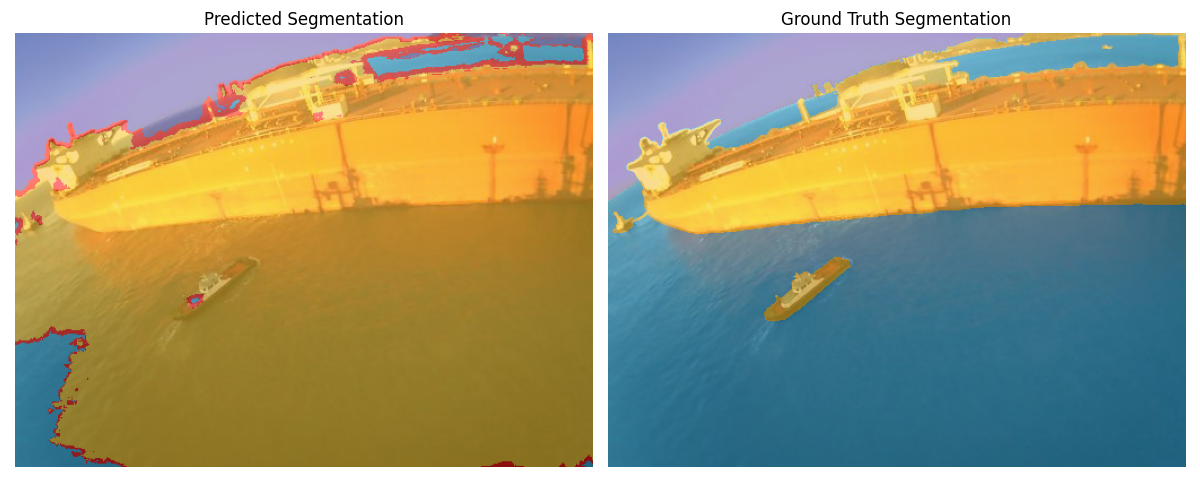
\includegraphics[width=0.99\textwidth]{figures/OASIs/SegNet-type1-23.png}
        \caption{}
    \end{subfigure}
    % subfig3
    \begin{subfigure}[h]{0.49\textwidth} \centering
        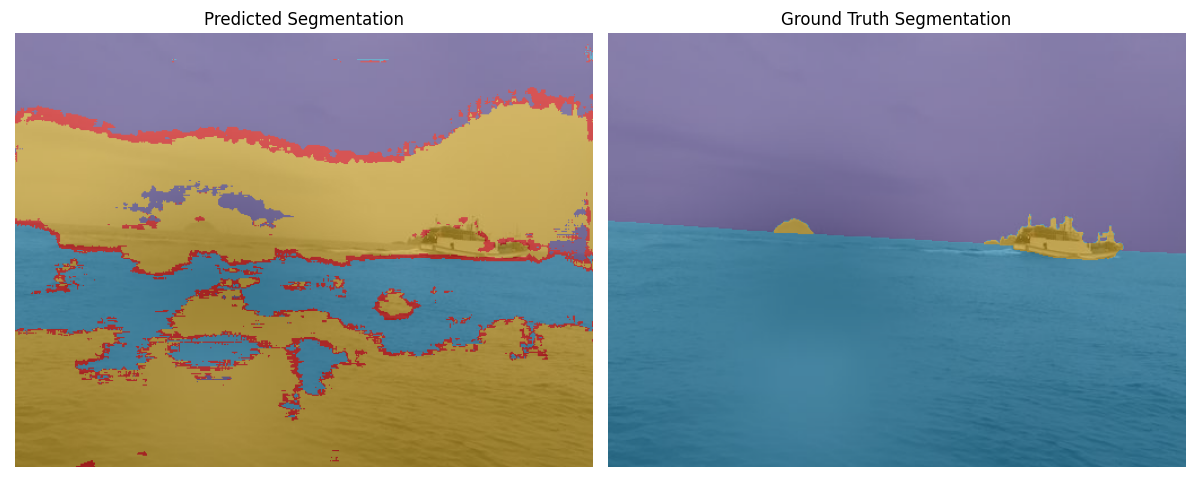
\includegraphics[width=0.99\textwidth]{figures/OASIs/SegNet-type2-29.png}
        \caption{}
    \end{subfigure} \hspace{-10mm}
    % subfig4
    \begin{subfigure}[h]{0.49\textwidth} \centering
        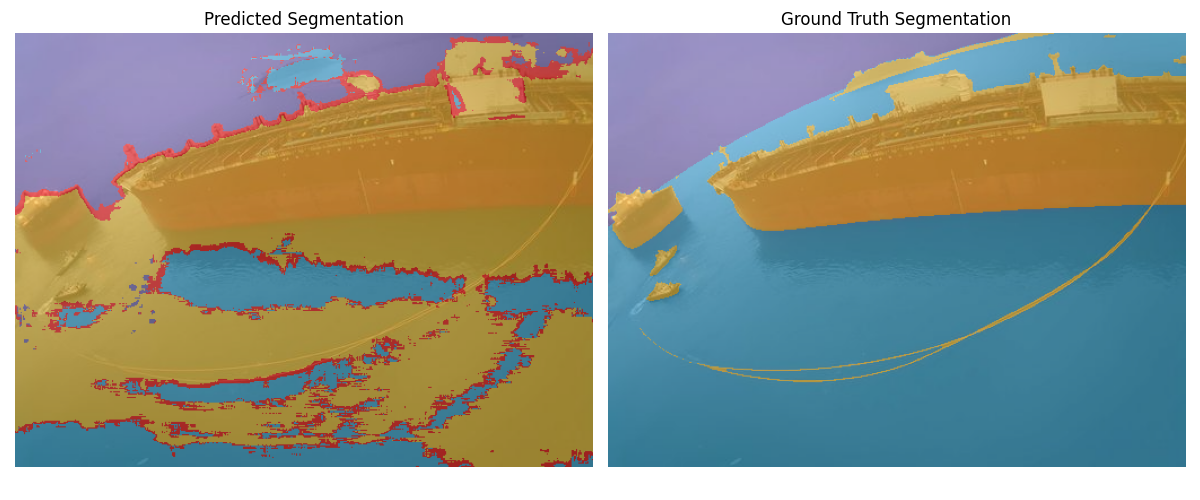
\includegraphics[width=0.99\textwidth]{figures/OASIs/SegNet-type2-24.png}
        \caption{}
    \end{subfigure}
    % subfig5
    \begin{subfigure}[h]{0.49\textwidth} \centering
        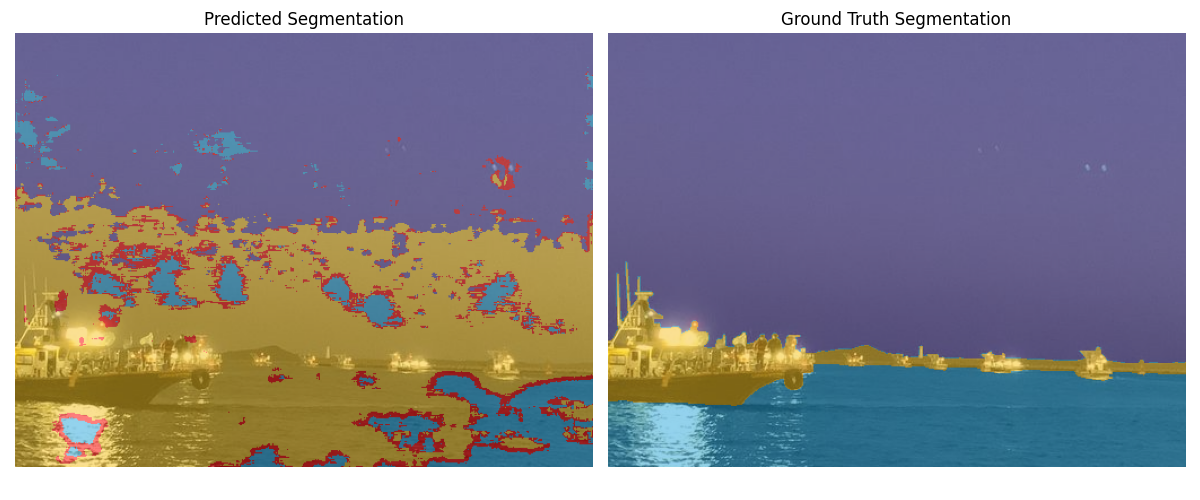
\includegraphics[width=0.99\textwidth]{figures/OASIs/SegNet-type3-53.png}
        \caption{}
    \end{subfigure} \hspace{-10mm}
    % subfig6
    \begin{subfigure}[h]{0.49\textwidth} \centering
        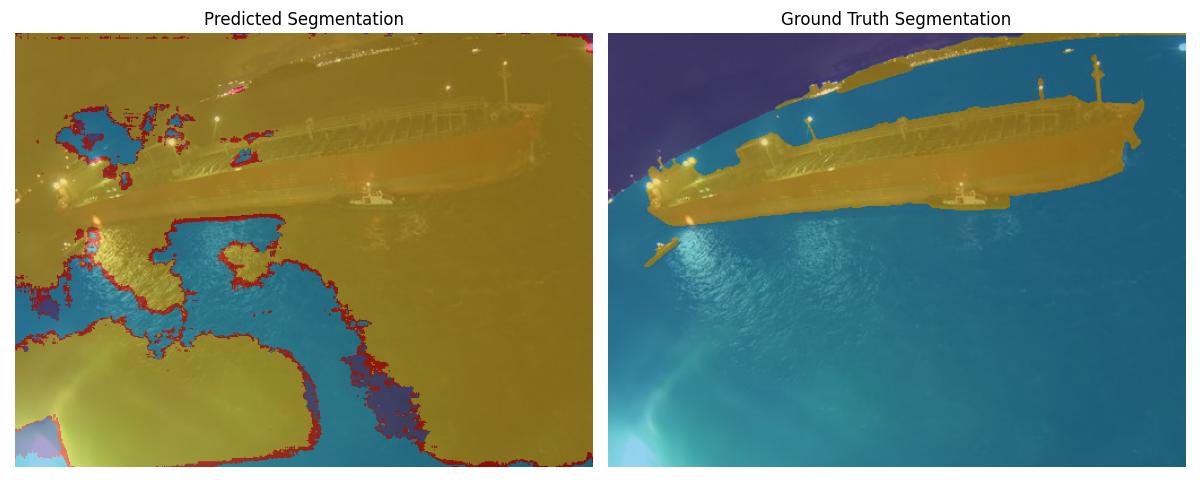
\includegraphics[width=0.99\textwidth]{figures/OASIs/SegNet-type3-18.png}
        \caption{}
    \end{subfigure}
    \caption{Semantic Segmentations of SegNet architecture on OASIs dataset: (a)type 1 with USV perspective, 
    (b)type 1 with cargo ship perspective, (c)type 2 with USV perspective, (d)type 2 with cargo ship perspective, 
    (e)type 3 with USV perspective, (f)type 3 with cargo ship perspective.}
    \label{fig:segnet-oasis}
\end{figure}

Regarding the SegNet architecture, the data from Table \ref{tab:DTEP} indicates that $\mathbf{Pr}$,  $\mathbf{Re}$, 
and  $\mathbf{F1}$ of subcategory type 1 from the USV perspectives are comparable to domain transfer analysis with 
SMD as a benchmark. However, for type 2 and 3, there is a notable decrease in $\mathbf{Pr}$ and a concurrent increase 
in $\mathbf{Re}$. This issue arises because SegNet labels a substantial number of pixels as class 0. While this 
results in high $\mathbf{TP_r}$ and low $\mathbf{FN_r}$, it also leads to a significant increase in $\mathbf{FP_r}$. 
In the cargo ship perspective, a similar issue of excessive labelling as class 0 is observed, as detailed in Fig.
\ref{fig:segnet-oasis}. Overall, the performance of SegNet on this dataset falls short of satisfactory segmentation.

Additionally, discrepancies due to different labelling standards also introduce errors. For example, as shown in 
Fig.\ref{fig:seagull}, in the MaSTR1325 dataset, seagulls are categorized as class 0, which is obstacles. However, 
according to the labelling standards of the OASIs dataset, they are not marked as sea objects in the ground truth. 
This discrepancy may also contribute to some degree of error. 
% figure
\begin{figure}[ht!]
    \centering
    % subfig1
    \begin{subfigure}[h]{0.45\textwidth} \centering
        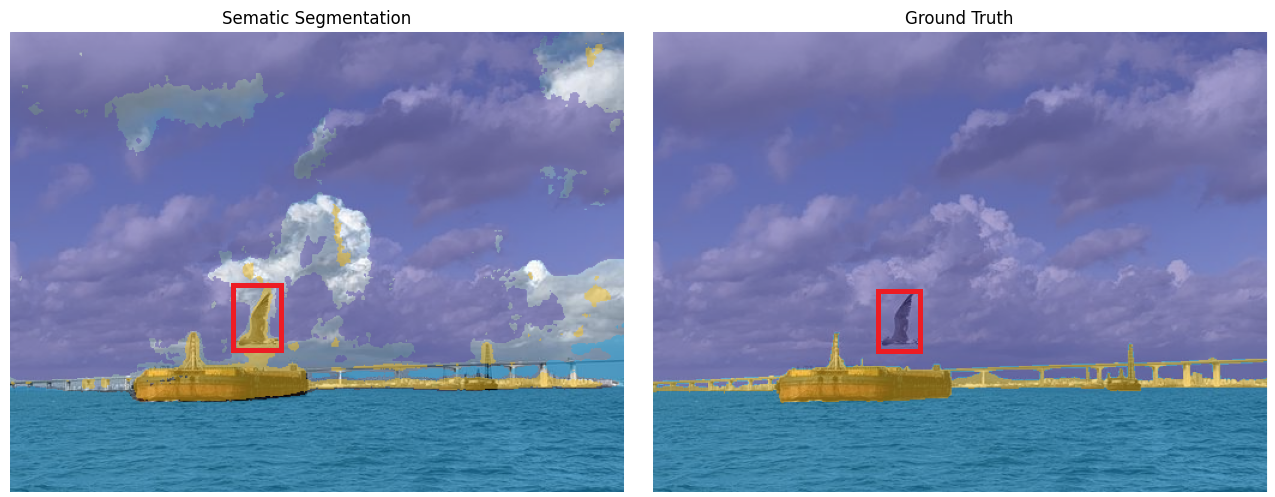
\includegraphics[width=0.99\textwidth]{figures/OASIs/BayesianSegNet-seagull.png}
        \caption{}
    \end{subfigure} \hspace{-1mm}
    % subfig2
    \begin{subfigure}[h]{0.45\textwidth} \centering
        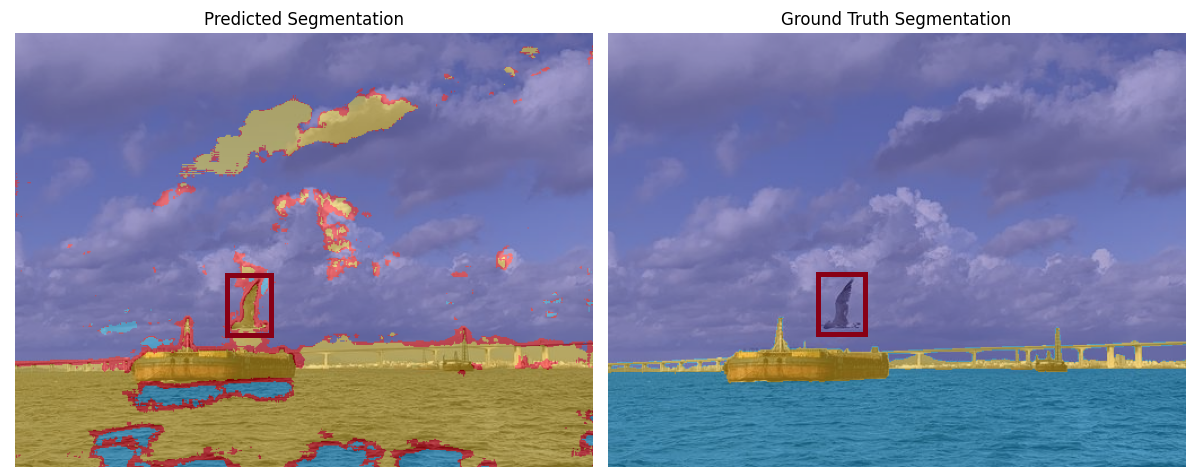
\includegraphics[width=0.99\textwidth]{figures/OASIs/SegNet-seagull.png}
        \caption{}
    \end{subfigure}
    \caption{Different labelling standards between MaSTr1325 and OASIs datasets: 
    (a) Seagulls Identified as Obstacles by Bayesian SegNet, (b) Seagulls Identified as Obstacles by SegNet.}
    \label{fig:seagull}
\end{figure}

Ultimately, further experiments are needed to fully assess the generalization capabilities of Bayesian SegNet. It 
would be beneficial to test the model using other datasets, such as SMD, and to apply various thresholds to filter 
the semantic segmentation results. Additionally, testing Bayesian and non-Bayesian models using the MODD2 dataset 
and associated tools could provide insights into their performance in water segmentation and Water-Edge Estimation 
Error in Pixels ($\mu_{edge}$). The current series of validations demonstrate the unique advantages of the model in 
enhancing the visual processing capabilities and robustness of USVs. However, they do not fully establish that the 
model can replace existing USV technologies or surpass other technologies in all respects.

